% Môn: Vật lý
% Lớp: 12
% Chương: Chương I. Vật lí nhiệt
% Bài: L12C1 Bài 6. Nhiệt hóa hơi riêng · Nhận biết và phân tích các quá trình chuyển thể
\dangbt{Nhận biết và phân tích các quá trình chuyển thể}
% ID: L12C1B1-TN-42
% Mức: NB
% ID: L12C1B1-91-TN


% ID: L12C1B1-TN-4
% Mức: NB
% ID: L12C1B1-97-TN
% ID: L12C1B1-97-TN
% Mức: NB
% ID: L12C1B1-97-TN
% Mức: NB
% ID: L12C1B1-97-TN


% ID: L12C1B1-TN-3
% Mức: NB
% ID: L12C1B1-100-TN
% ID: L12C1B1-100-TN
% Mức: NB
% ID: L12C1B1-100-TN
% Mức: NB
% ID: L12C1B1-100-TN
% ID: L12C1B1-100-TN
% Mức: NB
% ID: L12C1B1-100-TN
% Mức: NB
% ID: L12C1B1-100-TN


% ID: L12C1B1-TN-34
% Mức: TH
% ID: L12C1B1-102-TN
% ID: L12C1B1-102-TN
% Mức: TH
% ID: L12C1B1-102-TN
% Mức: TH
% ID: L12C1B1-102-TN
% ID: L12C1B1-102-TN
% Mức: TH
% ID: L12C1B1-102-TN
% Mức: TH
% ID: L12C1B1-102-TN
% ID: L12C1B1-102-TN
% Mức: TH
% ID: L12C1B6-91-TN
%=== Câu 12 ===%
\dangbt{Nhận biết và phân tích các quá trình chuyển thể}
\begin{ex}
% ID: L12C1B6-91-TN
% Mức: TH
	{\color{red}\footnotesize\ttfamily [L12C1B1-TN-34]}\par %HienID
	Trong thí nghiệm đo nhiệt hoá hơi riêng của nước sử dụng ấm đun siêu tốc, thao tác đặt ấm đun lên cân điện tử, hiệu chỉnh cân về số $0,00$ sau đó mới rót nước vào ấm đun là để
	\choice
	{cân khối lượng bình cho đơn giản}
	{số chỉ trên cân ổn định hơn}
	{an toàn và dễ tiến hành thí nghiệm hơn}
	{\True đo được chính xác và đồng thời khối lượng nước bay hơi và thời gian bay hơi tương ứng, phép đo đơn giản hơn}
	\loigiai{
		\begin{itemize}
			\item Thao tác đặt ấm đun lên cân điện tử, hiệu chỉnh cân về số $0{,}00$ sau đó mới rót nước vào ấm đun là để đo được chính xác và đồng thời khối lượng nước bay hơi và thời gian bay hơi tương ứng, phép đo đơn giản hơn.
		\end{itemize}
	}
\end{ex}

% ID: L12C1B1-TN-35
% Mức: TH
% ID: L12C1B1-103-TN
% ID: L12C1B1-103-TN
% Mức: TH
% ID: L12C1B1-103-TN
% Mức: TH
% ID: L12C1B1-103-TN
% ID: L12C1B1-103-TN
% Mức: TH
% ID: L12C1B1-103-TN
% Mức: TH
% ID: L12C1B1-103-TN
% ID: L12C1B1-103-TN
% Mức: TH
% ID: L12C1B6-92-TN
%=== Câu 13 ===%
\begin{ex}
% ID: L12C1B6-92-TN
% Mức: TH
	{\color{red}\footnotesize\ttfamily [L12C1B1-TN-35]}\par %HienID
	Để xác định nhiệt hóa hơi riêng của một số chất lỏng bằng thực nghiệm ta \textbf{không} cần dùng đến dụng cụ nào sau đây?
	\choice
	{Cân điện tử}
	{Nhiệt lượng kế}
	{Oát kế}
	{\True Vôn kế}
	\loigiai{
		\begin{itemize}
			\item Cần cân điện tử để xác định khối lượng nước đã bay hơi.
			\item Nhiệt lượng kế để giảm hao phí ra môi trường.
			\item Oát kế để xác định công suất của dòng điện.
			\item Từ đó xác định được nhiệt hóa hơi riêng $\dfrac{Pt}{\Delta m}$.
			\item Không cần dùng đến Vôn kế.
		\end{itemize}
	}
\end{ex}

% ID: L12C1B1-TN-38
% Mức: NB
% ID: L12C1B1-105-TN
% ID: L12C1B1-105-TN
% Mức: NB
% ID: L12C1B1-105-TN
% Mức: NB
% ID: L12C1B1-105-TN
% ID: L12C1B1-105-TN
% Mức: NB
% ID: L12C1B1-105-TN
% Mức: NB
% ID: L12C1B1-105-TN
% ID: L12C1B1-105-TN
% Mức: NB
% ID: L12C1B6-93-TN
%=== Câu 15 ===%
\begin{ex}
% ID: L12C1B6-93-TN
% Mức: NB
	{\color{red}\footnotesize\ttfamily [L12C1B1-TN-38]}\par %HienID
	Phát biểu nào sau đây là \textbf{sai}?
	\choice
	{\True Sự chuyển từ thể khí sang thể lỏng gọi là sự thăng hoa}
	{Sự chuyển từ thể rắn sang thể lỏng gọi là sự nóng chảy}
	{Sự chuyển từ thể lỏng sang thể rắn gọi là sự đông đặc}
	{Sự chuyển từ thể lỏng sang thể khí gọi là sự bay hơi}
	\loigiai{
		\begin{itemize}
			\item Sự chuyển từ thể khí sang thể lỏng gọi là ngưng tụ.
		\end{itemize}
	}
\end{ex}

% ID: L12C1B1-TN-41
% Mức: NB
% ID: L12C1B1-107-TN
% ID: L12C1B1-107-TN
% Mức: NB
% ID: L12C1B1-107-TN
% Mức: NB
% ID: L12C1B1-107-TN
% ID: L12C1B1-107-TN
% Mức: NB
% ID: L12C1B1-107-TN
% Mức: NB
% ID: L12C1B1-107-TN
% ID: L12C1B1-107-TN
% Mức: NB
% ID: L12C1B6-94-TN
%=== Câu 17 ===%
\begin{ex}
% ID: L12C1B6-94-TN
% Mức: NB
	{\color{red}\footnotesize\ttfamily [L12C1B1-TN-41]}\par %HienID
	Quá trình cục nước đá chuyển thành nước được gọi là quá trình
	\choice
	{đông đặc}
	{\True nóng chảy}
	{bay hơi}
	{ngưng kết}
	\loigiai{
		\begin{itemize}
			\item Quá trình cục nước đá chuyển thành nước được gọi là quá trình nóng chảy.
		\end{itemize}
	}
\end{ex}

% ID: L12C1B1-TN-1
% Mức: TH
% ID: L12C1B1-108-TN
% ID: L12C1B1-108-TN
% Mức: TH
% ID: L12C1B1-108-TN
% Mức: TH
% ID: L12C1B1-108-TN
% ID: L12C1B1-108-TN
% Mức: TH
% ID: L12C1B1-108-TN
% Mức: TH
% ID: L12C1B1-108-TN
% ID: L12C1B1-108-TN
% Mức: TH
% ID: L12C1B6-95-TN
%=== Câu 18 ===%
\begin{ex}
% ID: L12C1B6-95-TN
% Mức: TH
	{\color{red}\footnotesize\ttfamily [L12C1B1-TN-1]}\par %HienID
	Với cùng một chất, quá trình chuyển thể nào sẽ làm giảm lực tương tác giữa các phân tử nhiều nhất?
	\choice
	{Ngưng tụ}
	{Hóa hơi}
	{\True Thăng hoa}
	{Nóng chảy}
	\loigiai{
		\begin{itemize}
			\item Với cùng một chất, quá trình chuyển thể từ rắn sang hơi (thăng hoa) sẽ làm giảm lực tương tác giữa các phân tử nhiều nhất.
		\end{itemize}
	}
\end{ex}

% ID: L12C1B1-TN-5
% Mức: NB
% ID: L12C1B1-109-TN
% ID: L12C1B1-109-TN
% Mức: NB
% ID: L12C1B1-109-TN
% Mức: NB
% ID: L12C1B1-109-TN
% ID: L12C1B1-109-TN
% Mức: NB
% ID: L12C1B1-109-TN
% Mức: NB
% ID: L12C1B1-109-TN
% ID: L12C1B1-109-TN
% Mức: NB
% ID: L12C1B6-96-TN
%=== Câu 19 ===%
\begin{ex}
% ID: L12C1B6-96-TN
% Mức: NB
	{\color{red}\footnotesize\ttfamily [L12C1B1-TN-5]}\par %HienID
	Phát biểu nào sau đây là đúng về sự bay hơi?
	\choice
	{Sự bay hơi chỉ xảy ra khi chất lỏng đạt nhiệt độ sôi}
	{Sự bay hơi chỉ xảy ra khi chất lỏng có nhiệt độ thấp hơn nhiệt độ môi trường}
	{\True Sự bay hơi xảy ra ở nhiệt độ bất kì}
	{Tốc độ bay hơi không phụ thuộc vào nhiệt độ}
	\loigiai{\begin{enumerate}
			\item Sự hóa hơi trên bề mặt chất lõng là sự bay hơi.Sự bay hơi xảy ra ở nhiệt độ bất kì.
			\item tốc độ càng nhanh nếu diện tích mặt thoáng càng lớn
		\end{enumerate}
		Sự hóa hơi xảy ra trên bề mặt chất lỏng gọi là sự bay hơi. Sự bay hơi xảy ra ở nhiệt độ bất kì.}
\end{ex}

% ID: L12C1B1-TN-10
% Mức: NB
% ID: L12C1B1-111-TN
% ID: L12C1B1-111-TN
% Mức: NB
% ID: L12C1B1-111-TN
% Mức: NB
% ID: L12C1B1-111-TN
% ID: L12C1B1-111-TN
% Mức: NB
% ID: L12C1B1-111-TN
% Mức: NB
% ID: L12C1B1-111-TN
% ID: L12C1B1-111-TN
% Mức: NB
% ID: L12C1B6-97-TN
%=== Câu 21 ===%
\begin{ex}
% ID: L12C1B6-97-TN
% Mức: NB
	{\color{red}\footnotesize\ttfamily [L12C1B1-TN-10]}\par %HienID
	Nhiệt độ sôi của nước tinh khiết ở điều kiện áp suất tiêu chuẩn trong thang nhiệt độ Kelvin là
	\choice
	{$0\ \mathrm{K}$}
	{\True $373\ \mathrm{K}$}
	{$100\ \mathrm{K}$}
	{$273\ \mathrm{K}$}
	\loigiai{T(K)=t(C) +273 , nhiệt độ sôi của nước ở điều kiện tiêu chuẩn là 100 độ C đổi sang độ K:100+273=373K}
\end{ex}

% ID: L12C1B1-TN-12
% Mức: NB
% ID: L12C1B1-113-TN
% ID: L12C1B1-113-TN
% Mức: NB
% ID: L12C1B1-113-TN
% Mức: NB
% ID: L12C1B1-113-TN
% ID: L12C1B1-113-TN
% Mức: NB
% ID: L12C1B1-113-TN
% Mức: NB
% ID: L12C1B1-113-TN
% ID: L12C1B1-113-TN
% Mức: NB
% ID: L12C1B6-98-TN
%=== Câu 23 ===%
\begin{ex}
% ID: L12C1B6-98-TN
% Mức: NB
	{\color{red}\footnotesize\ttfamily [L12C1B1-TN-12]}\par %HienID
	Tốc độ bay hơi của chất lỏng \textbf{không} phụ thuộc trực tiếp vào yếu tố nào sau đây?
	\choice
	{\True thể tích của chất lỏng}
	{Diện tích mặt thoáng của chất lỏng}
	{Gió}
	{Nhiệt độ}
	\loigiai{Tốc độ bay hơi của chất lỏng càng nhanh nếu diện tích mặt thoáng càng lớn, tốc độ gió càng lớn, nhiệt độ càng cao, và độ ẩm không khí càng thấp.}
\end{ex}

% ID: L12C1B1-TN-15
% Mức: NB
% ID: L12C1B1-116-TN
% ID: L12C1B1-116-TN
% Mức: NB
% ID: L12C1B1-116-TN
% Mức: NB
% ID: L12C1B1-116-TN
% ID: L12C1B1-116-TN
% Mức: NB
% ID: L12C1B1-116-TN
% Mức: NB
% ID: L12C1B1-116-TN
% ID: L12C1B1-116-TN
% Mức: NB
% ID: L12C1B6-99-TN
%=== Câu 26 ===%
\begin{ex}
% ID: L12C1B6-99-TN
% Mức: NB
	{\color{red}\footnotesize\ttfamily [L12C1B1-TN-15]}\par %HienID
	Nước được đưa vào ngăn đá của tủ lạnh một thời gian sẽ chuyển thành nước đá. Sự chuyển thể của nước trong trường hợp này gọi là
	\choice
	{sự nóng chảy}
	{\True sự đông đặc}
	{sự ngưng tụ}
	{sự bay hơi}
	\loigiai{
		\begin{center}
			\resizebox{0.22\textwidth}{!}{
				\begin{tikzpicture}[>=Stealth, thick, font=\sffamily]
					
					\coordinate (RAN) at (0,0);
					\coordinate (LONG) at (5,0);
					\coordinate (KHI) at ($(RAN)!0.5!(LONG)+(0,4.33)$); % tam giác đều
					
					\shade[ball color=green!50!white] (RAN) circle (1.1cm);
					\node at (RAN) {\textbf{RẮN}};
					
					\shade[ball color=red!50!white] (LONG) circle (1.1cm);
					\node at (LONG) {\textbf{LỎNG}};
					
					\shade[ball color=cyan!50!white] (KHI) circle (1.1cm);
					\node at (KHI) {\textbf{KHÍ}};
					
					\draw[->, thick, green!60!black]
					($(RAN)+(1.1,0.3)$) -- ($(LONG)+(-1.1,0.3)$)
					node[midway, above, font=\small\bfseries, text=green!60!black] {nóng chảy};
					
					\draw[->, thick]
					($(LONG)+(-1.25,0)$) -- ($(RAN)+(1.25,0)$)
					node[midway, below, font=\small\bfseries] {đông đặc};
					
					\draw[->, thick, red!70!black]
					($(LONG)+(-0.6,1.0)$) -- ($(KHI)+(0.6,-1.0)$)
					node[midway, above, rotate=-60, font=\small\bfseries, text=red!70!black] {hoá hơi};
					
					\draw[->, thick]
					($(KHI)+(0.6,-1.4)$) -- ($(LONG)+(-0.8,0.9)$)
					node[midway, below, rotate=-65, font=\small\bfseries] {ngưng tụ};
					
					\draw[->, thick]
					($(RAN)+(0.6,1)$) -- ($(KHI)+(-0.7,-1.2)$)
					node[midway, above, rotate=60, font=\small\bfseries] {thăng hoa};
					
					\draw[->, thick, cyan!60!black]
					($(KHI)+(-0.6,-1.4)$) -- ($(RAN)+(0.8,0.9)$)
					node[midway, below, rotate=60, font=\small\bfseries, text=cyan!60!black] {ngưng kết};
					
				\end{tikzpicture}
			}
		\end{center}
	}
\end{ex}

% ID: L12C1B1-TN-18
% Mức: TH
% ID: L12C1B1-117-TN
% ID: L12C1B1-117-TN
% Mức: TH
% ID: L12C1B1-117-TN
% Mức: TH
% ID: L12C1B1-117-TN
% ID: L12C1B1-117-TN
% Mức: TH
% ID: L12C1B1-117-TN
% Mức: TH
% ID: L12C1B1-117-TN
% ID: L12C1B1-117-TN
% Mức: TH
% ID: L12C1B6-100-TN
%=== Câu 27 ===%
\begin{ex}
% ID: L12C1B6-100-TN
% Mức: TH
	{\color{red}\footnotesize\ttfamily [L12C1B1-TN-18]}\par %HienID
	Có 4 học sinh (HS) đưa ra các quan điểm về sự bay hơi như sau:
	\begin{enumerate}
		\item  HS1: Sự bay hơi là sự hóa hơi ở mặt thoáng chất lỏng ở nhiệt độ bất kì.
		\item HS2: Sự bay hơi diễn ra càng nhanh khi diện tích mặt thoáng càng lớn và tốc độ gió càng  mạnh.
		\item  HS3: Ở trên núi cao, tốc độ bay hơi của nước luôn diễn ra chậm hơn so với vùng đồng bằng.
		\item HS4: Đồng thời với sự bay hơi cũng có một số phân tử hơi bay ngược trở lại mặt thoáng để chuyển về thể lỏng, đó là sự ngưng tụ.
	\end{enumerate}
	Có bao nhiêu học sinh đưa ra quan điểm chính xác?
	\choice
	{$1$}
	{$2$}
	{\True $3$}
	{$4$}
	\loigiai{Sự hóa hơi xảy ra trên bề mặt chất lỏng gọi là sự bay hơi. Sự bay hơi xảy ra ở nhiệt độ bất kì. Tốc độ bay hơi của chất lỏng càng nhanh nếu diện tích mặt thoáng càng lớn, tốc độ gió càng lớn, nhiệt độ càng cao, và độ ẩm không khí càng thấp.}
\end{ex}

% ID: L12C1B1-TN-20
% Mức: TH
% ID: L12C1B1-119-TN
% ID: L12C1B1-119-TN
% Mức: TH
% ID: L12C1B1-119-TN
% Mức: TH
% ID: L12C1B1-119-TN
% ID: L12C1B1-119-TN
% Mức: TH
% ID: L12C1B1-119-TN
% Mức: TH
% ID: L12C1B1-119-TN
% ID: L12C1B1-119-TN
% Mức: TH
% ID: L12C1B6-101-TN
%=== Câu 29 ===%
\begin{ex}
% ID: L12C1B6-101-TN
% Mức: TH
	{\color{red}\footnotesize\ttfamily [L12C1B1-TN-20]}\par %HienID
	Nhiệt lượng mà chất rắn kết tinh hấp thụ trong quá trình nóng chảy chủ yếu được sử dụng để
	\choice
	{\True phá hủy cấu trúc mạng tinh thể và tăng động năng của các phân tử}
	{ phá hủy cấu trúc mạng tinh thể và tăng thế năng của các phân tử}
	{phá hủy cấu trúc mạng tinh thể và tăng động năng, thế năng của các phân tử}
	{phá hủy cấu trúc mạng tinh thể nhưng không làm tăng thế năng, động năng của các phân tử}
	\loigiai{
		\begin{itemchoice}
			\item Trong quá trình nóng chảy của chất rắn kết tinh, nhiệt lượng hấp thụ được dùng để phá vỡ các liên kết chặt chẽ giữa các phân tử trong mạng tinh thể. Đồng thời, năng lượng này giúp các phân tử chuyển động linh hoạt hơn (tăng động năng) để hệ chuyển từ trạng thái rắn sang trạng thái lỏng.
			\item Việc phá hủy mạng tinh thể làm thay đổi khoảng cách và sự tương tác giữa các phân tử (thế năng), nhưng để chuyển sang trạng thái lỏng cần sự tăng cường về khả năng chuyển động linh hoạt của các phân tử.
			\item Mặc dù quá trình này làm thay đổi nội năng của hệ (bao gồm cả động năng và thế năng phân tử), nhưng theo trọng tâm của đáp án đã cho, sự phá hủy cấu trúc và tăng động năng được nhấn mạnh là mục đích chính của việc hấp thụ nhiệt.
			\item Phương án này sai vì nhiệt lượng cung cấp cho hệ trong quá trình chuyển thể chắc chắn được dùng để phá hủy liên kết và làm thay đổi trạng thái năng lượng của các phân tử.
		\end{itemchoice}
	}
\end{ex}

% ID: L12C1B1-TN-23
% Mức: NB
% ID: L12C1B1-121-TN
% ID: L12C1B1-121-TN
% Mức: NB
% ID: L12C1B1-121-TN
% Mức: NB
% ID: L12C1B1-121-TN
% ID: L12C1B1-121-TN
% Mức: NB
% ID: L12C1B1-121-TN
% Mức: NB
% ID: L12C1B1-121-TN
% ID: L12C1B1-121-TN
% Mức: NB
% ID: L12C1B6-102-TN
%=== Câu 31 ===%
\begin{ex}
% ID: L12C1B6-102-TN
% Mức: NB
	{\color{red}\footnotesize\ttfamily [L12C1B1-TN-23]}\par %HienID
	Sự chuyển thể nào sau đây xảy ra ở một nhiệt độ xác định dưới một áp suất cho trước?
	\choice
	{Ngưng tụ}
	{Thăng hoa}
	{\True Sôi}
	{Bay hơi}
	
	\loigiai{
		\begin{itemize}
			\item Sự sôi xảy ra ở một nhiệt độ xác định dưới một áp suất cho trước.
	\end{itemize}}
\end{ex}

% ID: L12C1B1-TN-25
% Mức: NB
% ID: L12C1B1-123-TN
% ID: L12C1B1-123-TN
% Mức: NB
% ID: L12C1B1-123-TN
% Mức: NB
% ID: L12C1B1-123-TN
% ID: L12C1B1-123-TN
% Mức: NB
% ID: L12C1B1-123-TN
% Mức: NB
% ID: L12C1B1-123-TN
% ID: L12C1B1-123-TN
% Mức: NB
% ID: L12C1B6-103-TN
%=== Câu 33 ===%
\begin{ex}
% ID: L12C1B6-103-TN
% Mức: NB
	{\color{red}\footnotesize\ttfamily [L12C1B1-TN-25]}\par %HienID
	Quá trình một chất được chuyển từ thể rắn sang thể lỏng được gọi là quá trình
	\choice
	{hóa lỏng}
	{\True nóng chảy}
	{đông đặc}
	{hóa hơi}
	\loigiai{
		\begin{itemize}
			\item Quá trình một chất được chuyển từ thể rắn sang thể lỏng được gọi là quá trình nóng chảy.
	\end{itemize}}
\end{ex}

% ID: L12C1B1-TN-26
% Mức: NB
% ID: L12C1B1-124-TN
% ID: L12C1B1-124-TN
% Mức: NB
% ID: L12C1B1-124-TN
% Mức: NB
% ID: L12C1B1-124-TN
% ID: L12C1B1-124-TN
% Mức: NB
% ID: L12C1B1-124-TN
% Mức: NB
% ID: L12C1B1-124-TN
% ID: L12C1B1-124-TN
% Mức: NB
% ID: L12C1B6-104-TN
%=== Câu 34 ===%
\begin{ex}
% ID: L12C1B6-104-TN
% Mức: NB
	{\color{red}\footnotesize\ttfamily [L12C1B1-TN-26]}\par %HienID
	Quá trình một chất chuyển từ thể lỏng sang thể khí được gọi là quá trình
	\choice
	{\True hóa hơi}
	{đông đặc}
	{nóng chảy}
	{hóa lỏng}
	\loigiai{
		Quá trình một chất chuyên từ thể lỏng sang thể khí được gọi là quá trình hóa hơi.
		
	}
\end{ex}

% ID: L12C1B1-DS-3
% Mức: TH
% ID: L12C1B1-144-DS
% ID: L12C1B1-144-DS
% Mức: TH
% ID: L12C1B1-144-DS
% Mức: TH
% ID: L12C1B1-144-DS
% ID: L12C1B1-144-DS
% Mức: TH
% ID: L12C1B1-144-DS
% Mức: TH
% ID: L12C1B1-144-DS
% ID: L12C1B1-144-DS
% Mức: TH
% ID: L12C1B6-105-DS
%=== Câu 57 ===%
\begin{ex}
% ID: L12C1B6-105-DS
% Mức: TH
	{\color{red}\footnotesize\ttfamily [L12C1B1-DS-3]}\par %HienID
	Để đo nhiệt hóa hơi riêng của nước, cho các dụng cụ sau: Cân điện tử $(1)$, biến thế nguồn $(2)$, oát kế có tích hợp chức năng đo thời gian $(3)$, nhiệt lượng kế kèm dây điện trở $(4)$, nhiệt kế điện tử $(5)$ (hình vẽ).
	\begin{center}
		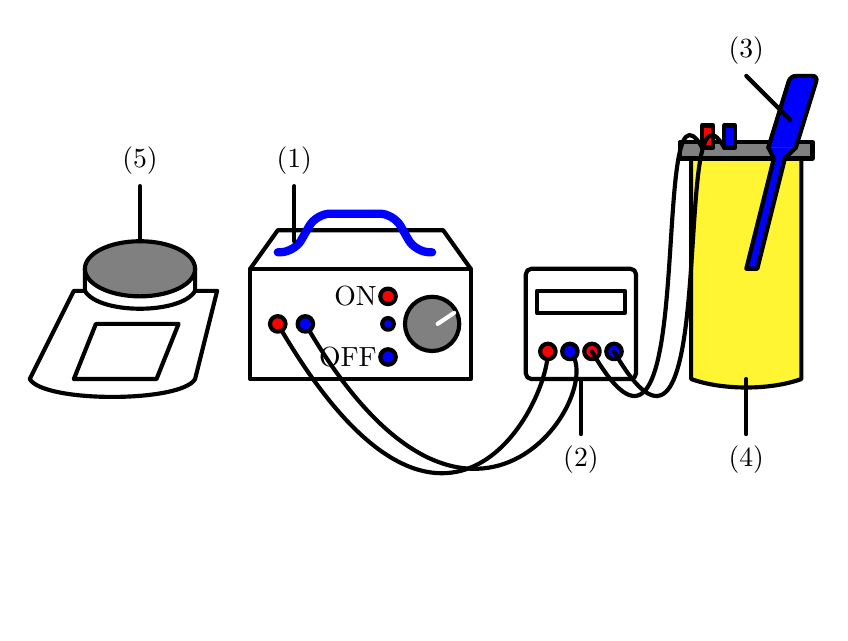
\begin{tikzpicture}[scale = 0.7, line join=round, line cap=round, >=stealth,line width=1.5]
			\draw[fill=gray](0,0) ellipse (1cm and 0.5cm);
			\draw (-1,0) -- (-1,-0.4) ..controls +(-60:0.5) and +(-120:0.5)..(1,-0.4) -- (1,0);
			\draw (-1,-0.4) -- (-1.2,-0.4) -- (-2,-2) ..controls +(-60:0.5) and +(-120:0.5).. (1,-2) -- (1.4,-0.4) -- (1,-0.4);
			\draw (-1.2,-2) -- (-0.8,-1) -- (0.7,-1) -- (0.3,-2) -- cycle;
			\draw (2,-2) rectangle (6,0);
			\draw (2,0) -- (2.5,0.7) -- (5.5,0.7) -- (6,0);
			\draw[rounded corners=2] (7,-2) rectangle (9,0);
			\draw (7.2,-0.8) rectangle (8.8,-0.4);
			\draw (2.5,-1) .. controls +(-60:6) and +(-90:1) ..(7.4,-1.5);
			\draw (3,-1) .. controls +(-60:6) and +(-45:1) ..(7.8,-1.5);
			\draw[fill=red] (2.5,-1) circle (4pt);
			\draw[fill=blue] (3,-1) circle (4pt);
			\draw[fill=red] (7.4,-1.5) circle (4pt);
			\draw[fill=blue] (7.8,-1.5) circle (4pt);
			\draw[fill=red] (8.2,-1.5) circle (4pt);
			\draw[fill=blue] (8.6,-1.5) circle (4pt);
			\draw[fill=gray] (5.3,-1) circle (14pt);
			\draw[white] (5.4,-1) -- (5.7,-0.8);
			\draw[fill=red] (4.5,-0.5) circle (4pt) node [left]{ON} ;
			\draw[fill=blue] (4.5,-1.6) circle (4pt) node [left]{OFF};
			\draw[fill=blue] (4.5,-1) circle (3pt);
			\draw[rounded corners=5,blue,line width=3] (2.5,0.3) -- (2.8,0.3) -- (3.2,1) -- (4.6,1) -- (5,0.3)-- (5.3,0.3);
			\draw[fill=yellow!80] (10,2) -- (10,-2) ..controls +(-20:0.6) and +(-160:0.6).. (12,-2)--(12,2);
			\draw[fill=gray] (9.8,2) rectangle (12.2,2.3);
			\draw[fill=red] (10.2,2.2) rectangle (10.4,2.6);
			\draw[fill=blue] (10.6,2.2) rectangle (10.8,2.6);
			\draw[rounded corners=2,fill=blue] (11.4,2.2) -- (11.8,3.5) -- (12.3,3.5) -- (11.9,2.2);
			\draw[fill=blue] (11.9,2.2) -- (11.7,2) -- (11.2,0) --(11,0)-- (11.5,2)--(11.4,2.2);
			\draw (8.2,-1.5) .. controls +(-60:4) and +(120:2).. (10.2,2.2);
			\draw (8.6,-1.5) .. controls +(-60:4) and +(120:2).. (10.6,2.2);
			\draw (0,0.5) -- (0,1.5) node [above] {(5)};
			\draw (2.8,0.5) -- (2.8,1.5) node [above] {(1)};
			\draw (8,-2) -- (8,-3) node [below] {(2)};
			\draw (11,-2) -- (11,-3) node [below] {(4)};
			\draw (11,3.5) node [above] {(3)} -- (11.8,2.7);
		\end{tikzpicture}
	\end{center}
	\choiceTF
	{\True Có thể sử dụng các dụng cụ trên để đo nhiệt hóa hơi riêng của nước ở nhiệt độ $100^\circ\mathrm{C}$}
	{\True Tiến hành thí nghiệm lần lượt theo các bước như sau: Đặt nhiệt lượng kế lên cân, đổ nước nóng vào nhiệt lượng kế sao cho toàn bộ dây điện trở chìm trong nước; Nối oát kế với nhiệt lượng kế và mở nắp nhiệt lượng kế; Xác định khối lượng nước trong bình; Bật nguồn điện, đun sôi nước trong nhiệt lượng kế; Quan sát ghi số chỉ trên đồng hồ đo thời gian, oát kế, cân vào bảng số liệu; Tắt nguồn}
	{Quan sát số chỉ trên cân, oát kế, đồng hồ đo thời gian thu được bảng số liệu như bảng dưới.\\
		\begin{center}
			\begin{tabular}{|c|c|c|c|c|c|c|c|c|}
				\hline
				$\tau\ (\ \mathrm{s})$ & 0 & 120 & 240 & 360 & 480 & 600 & 720 & 840 \\ 
				\hline
				$\mathcal{P}\ (\ \mathrm{W})$ & 0 & 15,21 & 15,19 & 15,21 & 15,23 & 15,19 & 15,21 & 15,19 \\ 
				\hline
				$m\ (\ \mathrm{kg})$ & 0,1200 & 0,1191 & 0,1184 & 0,1179 & 0,1170 & 0,1161 & 0,1152 & 0,1141 \\ 
				\hline
			\end{tabular}
		\end{center}
		Từ số liệu trên, vẽ được đồ thị khối lượng $m\ (\ \mathrm{kg})$ theo thời gian $\tau\ (\ \mathrm{s})$ có dạng đường thẳng đi qua gốc tọa độ.}
	{\True Từ số liệu trên, tính được nhiệt hóa hơi riêng của nước ở $100^\circ\mathrm{C}$ xấp xỉ là $2{,}3 \cdot 10^6\ \mathrm{J/kg}$}
	
	\loigiai{
		\begin{itemchoice}
			\item Các dụng cụ này cho phép xác định nhiệt lượng $Q$ cung cấp cho nước để hóa hơi (thông qua oát kế tích hợp chức năng đo thời gian) và khối lượng nước hóa hơi tương ứng $\Delta m$ (thông qua cân điện tử). Áp dụng công thức tính nhiệt hóa hơi: $L = \frac{Q}{\Delta m}$, ta có thể đo được nhiệt hóa hơi riêng của nước ở $100^\circ\mathrm{C}$.
			\item Quy trình thí nghiệm được mô tả chính xác các bước để đo sự biến thiên khối lượng của nước khi đang sôi dưới tác dụng của một công suất nhiệt không đổi từ dây điện trở. Việc mở nắp nhiệt lượng kế giúp hơi nước thoát ra ngoài để cân ghi nhận sự giảm khối lượng.
			\item Dựa vào bảng số liệu, tại thời điểm $\tau = 0\ \mathrm{s}$, khối lượng nước là $m = 0{,}1200\ \mathrm{kg} \neq 0$. Khi thời gian $\tau$ tăng, nước hóa hơi làm khối lượng $m$ giảm dần. Do đó, đồ thị khối lượng $m\ (\ \mathrm{kg})$ theo thời gian $\tau\ (\ \mathrm{s})$ có dạng là đường thẳng dốc xuống (hệ số góc âm) và không đi qua gốc tọa độ.
			\begin{center}
				\resizebox{0.28\textwidth}{!}{
					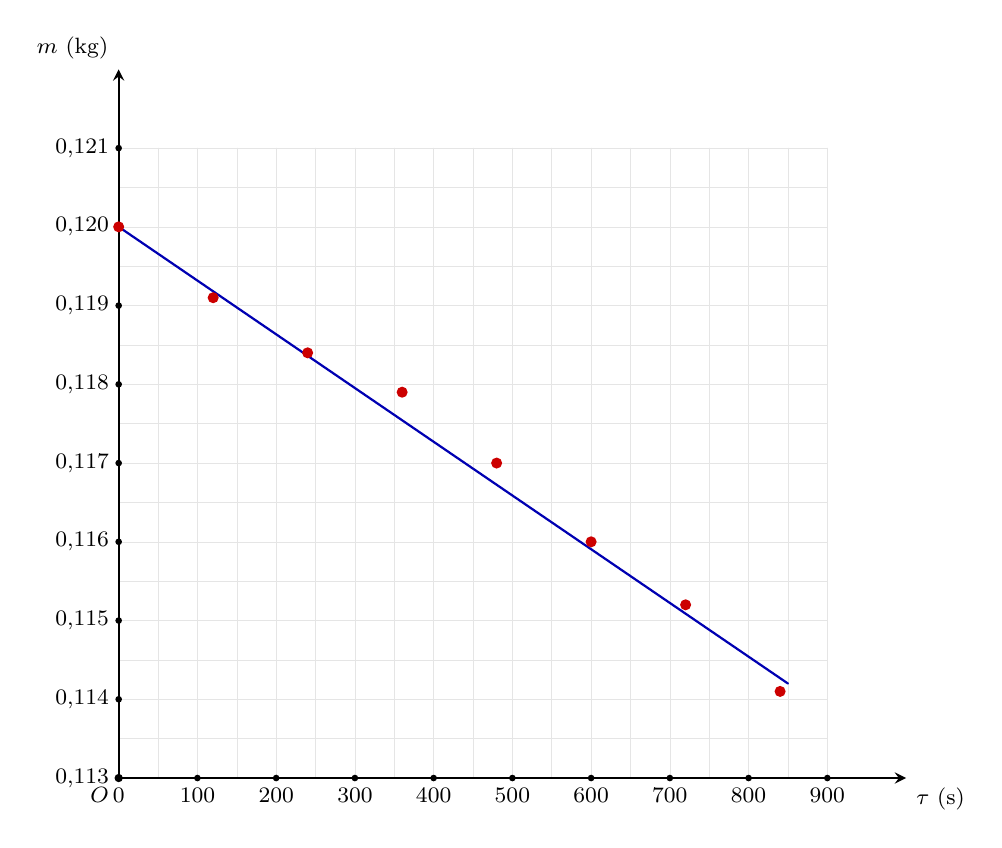
\begin{tikzpicture}[
						line join=round,
						line cap=round,
						>=stealth,
						font=\footnotesize
						]
						
				
						
						% Lưới
						\draw[step=0.5, gray!20, very thin] (0,0) grid (9,8);
						
						% Trục tọa độ
						\draw[->, thick] (0,0) -- (10,0) node[below right] {$\tau\ (\mathrm{s})$};
						\draw[->, thick] (0,0) -- (0,9) node[above left] {$m\ (\mathrm{kg})$};
						
						% Gốc tọa độ
						\fill (0,0) circle (1.5pt);
						\node[below left] at (0,0) {$O$};
						
						% Mốc trục Ox
						\foreach \x in {0,100,...,900}{
							\node[below] at ({\x/100},0) {\x};
							\fill ({\x/100},0) circle (1.2pt);
						}
						
						% Mốc trục Oy
						\foreach \y/\t in {
							0/0{,}113,
							1/0{,}114,
							2/0{,}115,
							3/0{,}116,
							4/0{,}117,
							5/0{,}118,
							6/0{,}119,
							7/0{,}120,
							8/0{,}121
						}{
							\node[left] at (0,\y) {\t};
							\fill (0,\y) circle (1.2pt);
						}
						
						% Đường xu hướng
						\draw[blue!70!black, thick] (0,7) -- (8.5,1.2);
						
						% Các điểm thực nghiệm
						\foreach \x/\y in {
							0/7,
							1.2/6.1,
							2.4/5.4,
							3.6/4.9,
							4.8/4,
							6/3,
							7.2/2.2,
							8.4/1.1
						}{
							\fill[red!80!black] (\x,\y) circle (2pt);
						}
						
					\end{tikzpicture}
				}
			\end{center}
			\item Áp dụng công thức tính công suất trung bình của dây điện trở:\\
			$$\overline{\mathcal{P}} = \frac{15{,}21+15{,}19+15{,}21+15{,}23+15{,}19+15{,}21+15{,}19}{7} \approx 15{,}204\ \mathrm{W}.$$
			Áp dụng công thức tính nhiệt lượng cung cấp cho nước hóa hơi: $Q = \overline{\mathcal{P}} \cdot \Delta \tau$.\\
			Áp dụng công thức tính nhiệt hóa hơi: $Q = L \cdot \Delta m \Rightarrow L = \frac{\overline{\mathcal{P}} \cdot \Delta \tau}{\Delta m}$.\\
			Chọn ra 2 điểm từ bảng số liệu: $\tau_1 = 0\ \mathrm{s} \Rightarrow m_1 = 0{,}1200\ \mathrm{kg}$ và $\tau_2 = 240\ \mathrm{s} \Rightarrow m_2 = 0{,}1184\ \mathrm{kg}$.\\
			Độ giảm khối lượng: $\Delta m = m_1 - m_2 = 0{,}1200 - 0{,}1184 = 0{,}0016\ \mathrm{kg}$.\\
			Nhiệt hóa hơi riêng đo được là: 
			$L = \frac{15{,}204 \cdot (240 - 0)}{0{,}0016} \approx 2\,280\,600\ \mathrm{J/kg} \approx 2{,}3 \cdot 10^6\ \mathrm{J/kg}$.
		\end{itemchoice}
	}
\end{ex}

% ===== Câu 49 =====
% ID: L12C1B6-106-DS
% Mức: NB
\begin{ex}
% ID: L12C1B6-106-DS
% Mức: NB
Xét các phát biểu sau về dạng “Nhận biết và phân tích các quá trình chuyển thể” (bộ số 4).
\choiceTF
{\True Nóng chảy là quá trình chuyển từ thể rắn sang thể lỏng.}
{Ngưng tụ là quá trình chuyển trực tiếp từ thể rắn sang thể khí.}
{\True Khi giải dạng “Nhận biết và phân tích các quá trình chuyển thể”, cần xác định đúng trạng thái đầu, trạng thái cuối và quy ước dấu hoặc điều kiện áp dụng.}
{Có thể bỏ qua mọi dữ kiện về khối lượng, nhiệt độ và hiệu suất trong mọi bài toán thuộc dạng này.}
\loigiai{
\begin{itemchoice}
\item (Đúng) Nóng chảy là quá trình chuyển từ thể rắn sang thể lỏng. (Vì): Nóng chảy là quá trình chuyển từ thể rắn sang thể lỏng. b) S: Ngưng tụ là quá trình chuyển trực tiếp từ thể rắn sang thể khí. c) Đ: Khi giải dạng “Nhận biết và phân tích các quá trình chuyển thể”, cần xác định đúng trạng thái đầu, trạng thái cuối và quy ước dấu hoặc điều kiện áp dụng. d) S: Có thể bỏ qua mọi dữ kiện về khối lượng, nhiệt độ và hiệu suất trong mọi bài toán thuộc dạng này. Kết luận dựa trên định nghĩa, điều kiện áp dụng và quy ước trong SGK KNTT
\item (Sai) Ngưng tụ là quá trình chuyển trực tiếp từ thể rắn sang thể khí.
\item (Đúng) Khi giải dạng “Nhận biết và phân tích các quá trình chuyển thể”, cần xác định đúng trạng thái đầu, trạng thái cuối và quy ước dấu hoặc điều kiện áp dụng.
\item (Sai) Có thể bỏ qua mọi dữ kiện về khối lượng, nhiệt độ và hiệu suất trong mọi bài toán thuộc dạng này.
\end{itemchoice}
}
\end{ex}

% ===== Câu 50 =====
% ID: L12C1B6-107-TL
% Mức: NB
\begin{bt}
% ID: L12C1B6-107-TL
% Mức: NB
Trình bày cách nhận biết và phương pháp giải dạng “Nhận biết và phân tích các quá trình chuyển thể”. Phân tích nhận định sau và sửa lại nếu sai: “Ngưng tụ là quá trình chuyển trực tiếp từ thể rắn sang thể khí.”
\loigiai{
Trước hết xác định hiện tượng, trạng thái và các đại lượng đã cho. Nêu định nghĩa hoặc hệ thức phù hợp, đổi về đơn vị SI, áp dụng đúng điều kiện và kiểm tra ý nghĩa kết quả. Nhận định cần đối chiếu: Nóng chảy là quá trình chuyển từ thể rắn sang thể lỏng. Vì vậy nhận định đã cho sai; phát biểu đúng là: Nóng chảy là quá trình chuyển từ thể rắn sang thể lỏng.
}
\end{bt}

% ===== Câu 51 =====
% ID: L12C1B6-108-TLN
% Mức: NB
\begin{ex}
% ID: L12C1B6-108-TLN
% Mức: NB
Cho bốn nhận định: (1) Nóng chảy là quá trình chuyển từ thể rắn sang thể lỏng. (2) Ngưng tụ là quá trình chuyển trực tiếp từ thể rắn sang thể khí. (3) Cần kiểm tra đơn vị và điều kiện áp dụng khi xử lí dạng “Nhận biết và phân tích các quá trình chuyển thể”. (4) Có thể thay tùy ý nhiệt độ Celsius cho nhiệt độ tuyệt đối trong mọi công thức. Có bao nhiêu nhận định đúng? Trả lời bằng một số nguyên.
\shortans{2}
\loigiai{
Nhận định (1) và (3) đúng; (2) và (4) sai. Vậy có 2 nhận định đúng.
}
\end{ex}

% ===== Câu 53 =====
% ID: L12C1B6-109-DS
% Mức: TH
\begin{ex}
% ID: L12C1B6-109-DS
% Mức: TH
Xét các phát biểu sau về dạng “Nhận biết và phân tích các quá trình chuyển thể” (bộ số 1).
\choiceTF
{Ngưng tụ là quá trình chuyển trực tiếp từ thể rắn sang thể khí.}
{\True Khi giải dạng “Nhận biết và phân tích các quá trình chuyển thể”, cần xác định đúng trạng thái đầu, trạng thái cuối và quy ước dấu hoặc điều kiện áp dụng.}
{Có thể bỏ qua mọi dữ kiện về khối lượng, nhiệt độ và hiệu suất trong mọi bài toán thuộc dạng này.}
{\True Nóng chảy là quá trình chuyển từ thể rắn sang thể lỏng.}
\loigiai{
\begin{itemchoice}
\item (Sai) Ngưng tụ là quá trình chuyển trực tiếp từ thể rắn sang thể khí. (Vì): Ngưng tụ là quá trình chuyển trực tiếp từ thể rắn sang thể khí. b) Đ: Khi giải dạng “Nhận biết và phân tích các quá trình chuyển thể”, cần xác định đúng trạng thái đầu, trạng thái cuối và quy ước dấu hoặc điều kiện áp dụng. c) S: Có thể bỏ qua mọi dữ kiện về khối lượng, nhiệt độ và hiệu suất trong mọi bài toán thuộc dạng này. d) Đ: Nóng chảy là quá trình chuyển từ thể rắn sang thể lỏng. Kết luận dựa trên định nghĩa, điều kiện áp dụng và quy ước trong SGK KNTT
\item (Đúng) Khi giải dạng “Nhận biết và phân tích các quá trình chuyển thể”, cần xác định đúng trạng thái đầu, trạng thái cuối và quy ước dấu hoặc điều kiện áp dụng.
\item (Sai) Có thể bỏ qua mọi dữ kiện về khối lượng, nhiệt độ và hiệu suất trong mọi bài toán thuộc dạng này.
\item (Đúng) Nóng chảy là quá trình chuyển từ thể rắn sang thể lỏng.
\end{itemchoice}
}
\end{ex}

% ===== Câu 57 =====
% ID: L12C1B6-110-DS
% Mức: TH
\begin{ex}
% ID: L12C1B6-110-DS
% Mức: TH
Xét các phát biểu sau về dạng “Nhận biết và phân tích các quá trình chuyển thể” (bộ số 5).
\choiceTF
{Ngưng tụ là quá trình chuyển trực tiếp từ thể rắn sang thể khí.}
{\True Khi giải dạng “Nhận biết và phân tích các quá trình chuyển thể”, cần xác định đúng trạng thái đầu, trạng thái cuối và quy ước dấu hoặc điều kiện áp dụng.}
{Có thể bỏ qua mọi dữ kiện về khối lượng, nhiệt độ và hiệu suất trong mọi bài toán thuộc dạng này.}
{\True Nóng chảy là quá trình chuyển từ thể rắn sang thể lỏng.}
\loigiai{
\begin{itemchoice}
\item (Sai) Ngưng tụ là quá trình chuyển trực tiếp từ thể rắn sang thể khí. (Vì): Ngưng tụ là quá trình chuyển trực tiếp từ thể rắn sang thể khí. b) Đ: Khi giải dạng “Nhận biết và phân tích các quá trình chuyển thể”, cần xác định đúng trạng thái đầu, trạng thái cuối và quy ước dấu hoặc điều kiện áp dụng. c) S: Có thể bỏ qua mọi dữ kiện về khối lượng, nhiệt độ và hiệu suất trong mọi bài toán thuộc dạng này. d) Đ: Nóng chảy là quá trình chuyển từ thể rắn sang thể lỏng. Kết luận dựa trên định nghĩa, điều kiện áp dụng và quy ước trong SGK KNTT
\item (Đúng) Khi giải dạng “Nhận biết và phân tích các quá trình chuyển thể”, cần xác định đúng trạng thái đầu, trạng thái cuối và quy ước dấu hoặc điều kiện áp dụng.
\item (Sai) Có thể bỏ qua mọi dữ kiện về khối lượng, nhiệt độ và hiệu suất trong mọi bài toán thuộc dạng này.
\item (Đúng) Nóng chảy là quá trình chuyển từ thể rắn sang thể lỏng.
\end{itemchoice}
}
\end{ex}

% ===== Câu 58 =====
% ID: L12C1B6-111-TL
% Mức: TH
\begin{bt}
% ID: L12C1B6-111-TL
% Mức: TH
Trình bày cách nhận biết và phương pháp giải dạng “Nhận biết và phân tích các quá trình chuyển thể”. Phân tích nhận định sau và sửa lại nếu sai: “Nóng chảy là quá trình chuyển từ thể rắn sang thể lỏng.”
\loigiai{
Trước hết xác định hiện tượng, trạng thái và các đại lượng đã cho. Nêu định nghĩa hoặc hệ thức phù hợp, đổi về đơn vị SI, áp dụng đúng điều kiện và kiểm tra ý nghĩa kết quả. Nhận định cần đối chiếu: Nóng chảy là quá trình chuyển từ thể rắn sang thể lỏng. Vì vậy nhận định đã cho đúng.
}
\end{bt}

% ===== Câu 61 =====
% ID: L12C1B6-112-DS
% Mức: VD
\begin{ex}
% ID: L12C1B6-112-DS
% Mức: VD
Xét các phát biểu sau về dạng “Nhận biết và phân tích các quá trình chuyển thể” (bộ số 2).
\choiceTF
{\True Khi giải dạng “Nhận biết và phân tích các quá trình chuyển thể”, cần xác định đúng trạng thái đầu, trạng thái cuối và quy ước dấu hoặc điều kiện áp dụng.}
{Có thể bỏ qua mọi dữ kiện về khối lượng, nhiệt độ và hiệu suất trong mọi bài toán thuộc dạng này.}
{\True Nóng chảy là quá trình chuyển từ thể rắn sang thể lỏng.}
{Ngưng tụ là quá trình chuyển trực tiếp từ thể rắn sang thể khí.}
\loigiai{
\begin{itemchoice}
\item (Đúng) Khi giải dạng “Nhận biết và phân tích các quá trình chuyển thể”, cần xác định đúng trạng thái đầu, trạng thái cuối và quy ước dấu hoặc điều kiện áp dụng. (Vì): Khi giải dạng “Nhận biết và phân tích các quá trình chuyển thể”, cần xác định đúng trạng thái đầu, trạng thái cuối và quy ước dấu hoặc điều kiện áp dụng. b) S: Có thể bỏ qua mọi dữ kiện về khối lượng, nhiệt độ và hiệu suất trong mọi bài toán thuộc dạng này. c) Đ: Nóng chảy là quá trình chuyển từ thể rắn sang thể lỏng. d) S: Ngưng tụ là quá trình chuyển trực tiếp từ thể rắn sang thể khí. Kết luận dựa trên định nghĩa, điều kiện áp dụng và quy ước trong SGK KNTT
\item (Sai) Có thể bỏ qua mọi dữ kiện về khối lượng, nhiệt độ và hiệu suất trong mọi bài toán thuộc dạng này.
\item (Đúng) Nóng chảy là quá trình chuyển từ thể rắn sang thể lỏng.
\item (Sai) Ngưng tụ là quá trình chuyển trực tiếp từ thể rắn sang thể khí.
\end{itemchoice}
}
\end{ex}

% ===== Câu 65 =====
% ID: L12C1B6-113-DS
% Mức: VDC
\begin{ex}
% ID: L12C1B6-113-DS
% Mức: VDC
Xét các phát biểu sau về dạng “Nhận biết và phân tích các quá trình chuyển thể” (bộ số 3).
\choiceTF
{Có thể bỏ qua mọi dữ kiện về khối lượng, nhiệt độ và hiệu suất trong mọi bài toán thuộc dạng này.}
{\True Nóng chảy là quá trình chuyển từ thể rắn sang thể lỏng.}
{Ngưng tụ là quá trình chuyển trực tiếp từ thể rắn sang thể khí.}
{\True Khi giải dạng “Nhận biết và phân tích các quá trình chuyển thể”, cần xác định đúng trạng thái đầu, trạng thái cuối và quy ước dấu hoặc điều kiện áp dụng.}
\loigiai{
\begin{itemchoice}
\item (Sai) Có thể bỏ qua mọi dữ kiện về khối lượng, nhiệt độ và hiệu suất trong mọi bài toán thuộc dạng này. (Vì): Có thể bỏ qua mọi dữ kiện về khối lượng, nhiệt độ và hiệu suất trong mọi bài toán thuộc dạng này. b) Đ: Nóng chảy là quá trình chuyển từ thể rắn sang thể lỏng. c) S: Ngưng tụ là quá trình chuyển trực tiếp từ thể rắn sang thể khí. d) Đ: Khi giải dạng “Nhận biết và phân tích các quá trình chuyển thể”, cần xác định đúng trạng thái đầu, trạng thái cuối và quy ước dấu hoặc điều kiện áp dụng. Kết luận dựa trên định nghĩa, điều kiện áp dụng và quy ước trong SGK KNTT
\item (Đúng) Nóng chảy là quá trình chuyển từ thể rắn sang thể lỏng.
\item (Sai) Ngưng tụ là quá trình chuyển trực tiếp từ thể rắn sang thể khí.
\item (Đúng) Khi giải dạng “Nhận biết và phân tích các quá trình chuyển thể”, cần xác định đúng trạng thái đầu, trạng thái cuối và quy ước dấu hoặc điều kiện áp dụng.
\end{itemchoice}
}
\end{ex}

% ===== Câu 155 =====
% ID: L12C1B6-114-TN
% Mức: NB
\begin{ex}
% ID: L12C1B6-114-TN
% Mức: NB
Câu 1 thuộc dạng “Nhận biết và phân tích các quá trình chuyển thể”. Phát biểu nào sau đây đúng?
\choice
{Ngưng tụ là quá trình chuyển trực tiếp từ thể rắn sang thể khí.}
{Nhiệt lượng và nhiệt độ là hai đại lượng hoàn toàn giống nhau.}
{Mọi quá trình nhiệt học đều không phụ thuộc điều kiện thực hiện.}
{\True Nóng chảy là quá trình chuyển từ thể rắn sang thể lỏng.}
\loigiai{
Phát biểu đúng là: Nóng chảy là quá trình chuyển từ thể rắn sang thể lỏng. Các phương án còn lại trái với mô hình, định nghĩa hoặc hệ thức nhiệt học tương ứng.
}
\end{ex}

% ===== Câu 156 =====
% ID: L12C1B6-115-TN
% Mức: NB
\begin{ex}
% ID: L12C1B6-115-TN
% Mức: NB
Câu 5 thuộc dạng “Nhận biết và phân tích các quá trình chuyển thể”. Phát biểu nào sau đây đúng?
\choice
{Ngưng tụ là quá trình chuyển trực tiếp từ thể rắn sang thể khí.}
{Nhiệt lượng và nhiệt độ là hai đại lượng hoàn toàn giống nhau.}
{Mọi quá trình nhiệt học đều không phụ thuộc điều kiện thực hiện.}
{\True Nóng chảy là quá trình chuyển từ thể rắn sang thể lỏng.}
\loigiai{
Phát biểu đúng là: Nóng chảy là quá trình chuyển từ thể rắn sang thể lỏng. Các phương án còn lại trái với mô hình, định nghĩa hoặc hệ thức nhiệt học tương ứng.
}
\end{ex}

% ===== Câu 157 =====
% ID: L12C1B6-116-TN
% Mức: NB
\begin{ex}
% ID: L12C1B6-116-TN
% Mức: NB
Câu 9 thuộc dạng “Nhận biết và phân tích các quá trình chuyển thể”. Phát biểu nào sau đây đúng?
\choice
{Ngưng tụ là quá trình chuyển trực tiếp từ thể rắn sang thể khí.}
{Nhiệt lượng và nhiệt độ là hai đại lượng hoàn toàn giống nhau.}
{Mọi quá trình nhiệt học đều không phụ thuộc điều kiện thực hiện.}
{\True Nóng chảy là quá trình chuyển từ thể rắn sang thể lỏng.}
\loigiai{
Phát biểu đúng là: Nóng chảy là quá trình chuyển từ thể rắn sang thể lỏng. Các phương án còn lại trái với mô hình, định nghĩa hoặc hệ thức nhiệt học tương ứng.
}
\end{ex}

% ===== Câu 158 =====
% ID: L12C1B6-117-TN
% Mức: TH
\begin{ex}
% ID: L12C1B6-117-TN
% Mức: TH
Câu 2 thuộc dạng “Nhận biết và phân tích các quá trình chuyển thể”. Phát biểu nào sau đây đúng?
\choice
{Nhiệt lượng và nhiệt độ là hai đại lượng hoàn toàn giống nhau.}
{Mọi quá trình nhiệt học đều không phụ thuộc điều kiện thực hiện.}
{\True Nóng chảy là quá trình chuyển từ thể rắn sang thể lỏng.}
{Ngưng tụ là quá trình chuyển trực tiếp từ thể rắn sang thể khí.}
\loigiai{
Phát biểu đúng là: Nóng chảy là quá trình chuyển từ thể rắn sang thể lỏng. Các phương án còn lại trái với mô hình, định nghĩa hoặc hệ thức nhiệt học tương ứng.
}
\end{ex}

% ===== Câu 159 =====
% ID: L12C1B6-118-TN
% Mức: TH
\begin{ex}
% ID: L12C1B6-118-TN
% Mức: TH
Câu 6 thuộc dạng “Nhận biết và phân tích các quá trình chuyển thể”. Phát biểu nào sau đây đúng?
\choice
{Nhiệt lượng và nhiệt độ là hai đại lượng hoàn toàn giống nhau.}
{Mọi quá trình nhiệt học đều không phụ thuộc điều kiện thực hiện.}
{\True Nóng chảy là quá trình chuyển từ thể rắn sang thể lỏng.}
{Ngưng tụ là quá trình chuyển trực tiếp từ thể rắn sang thể khí.}
\loigiai{
Phát biểu đúng là: Nóng chảy là quá trình chuyển từ thể rắn sang thể lỏng. Các phương án còn lại trái với mô hình, định nghĩa hoặc hệ thức nhiệt học tương ứng.
}
\end{ex}

% ===== Câu 160 =====
% ID: L12C1B6-119-TN
% Mức: TH
\begin{ex}
% ID: L12C1B6-119-TN
% Mức: TH
Câu 10 thuộc dạng “Nhận biết và phân tích các quá trình chuyển thể”. Phát biểu nào sau đây đúng?
\choice
{Nhiệt lượng và nhiệt độ là hai đại lượng hoàn toàn giống nhau.}
{Mọi quá trình nhiệt học đều không phụ thuộc điều kiện thực hiện.}
{\True Nóng chảy là quá trình chuyển từ thể rắn sang thể lỏng.}
{Ngưng tụ là quá trình chuyển trực tiếp từ thể rắn sang thể khí.}
\loigiai{
Phát biểu đúng là: Nóng chảy là quá trình chuyển từ thể rắn sang thể lỏng. Các phương án còn lại trái với mô hình, định nghĩa hoặc hệ thức nhiệt học tương ứng.
}
\end{ex}

% ===== Câu 161 =====
% ID: L12C1B6-120-TN
% Mức: VD
\begin{ex}
% ID: L12C1B6-120-TN
% Mức: VD
Câu 3 thuộc dạng “Nhận biết và phân tích các quá trình chuyển thể”. Phát biểu nào sau đây đúng?
\choice
{Mọi quá trình nhiệt học đều không phụ thuộc điều kiện thực hiện.}
{\True Nóng chảy là quá trình chuyển từ thể rắn sang thể lỏng.}
{Ngưng tụ là quá trình chuyển trực tiếp từ thể rắn sang thể khí.}
{Nhiệt lượng và nhiệt độ là hai đại lượng hoàn toàn giống nhau.}
\loigiai{
Phát biểu đúng là: Nóng chảy là quá trình chuyển từ thể rắn sang thể lỏng. Các phương án còn lại trái với mô hình, định nghĩa hoặc hệ thức nhiệt học tương ứng.
}
\end{ex}

% ===== Câu 162 =====
% ID: L12C1B6-121-TN
% Mức: VD
\begin{ex}
% ID: L12C1B6-121-TN
% Mức: VD
Câu 7 thuộc dạng “Nhận biết và phân tích các quá trình chuyển thể”. Phát biểu nào sau đây đúng?
\choice
{Mọi quá trình nhiệt học đều không phụ thuộc điều kiện thực hiện.}
{\True Nóng chảy là quá trình chuyển từ thể rắn sang thể lỏng.}
{Ngưng tụ là quá trình chuyển trực tiếp từ thể rắn sang thể khí.}
{Nhiệt lượng và nhiệt độ là hai đại lượng hoàn toàn giống nhau.}
\loigiai{
Phát biểu đúng là: Nóng chảy là quá trình chuyển từ thể rắn sang thể lỏng. Các phương án còn lại trái với mô hình, định nghĩa hoặc hệ thức nhiệt học tương ứng.
}
\end{ex}

% ===== Câu 163 =====
% ID: L12C1B6-122-TN
% Mức: VDC
\begin{ex}
% ID: L12C1B6-122-TN
% Mức: VDC
Câu 4 thuộc dạng “Nhận biết và phân tích các quá trình chuyển thể”. Phát biểu nào sau đây đúng?
\choice
{\True Nóng chảy là quá trình chuyển từ thể rắn sang thể lỏng.}
{Ngưng tụ là quá trình chuyển trực tiếp từ thể rắn sang thể khí.}
{Nhiệt lượng và nhiệt độ là hai đại lượng hoàn toàn giống nhau.}
{Mọi quá trình nhiệt học đều không phụ thuộc điều kiện thực hiện.}
\loigiai{
Phát biểu đúng là: Nóng chảy là quá trình chuyển từ thể rắn sang thể lỏng. Các phương án còn lại trái với mô hình, định nghĩa hoặc hệ thức nhiệt học tương ứng.
}
\end{ex}

% ===== Câu 164 =====
% ID: L12C1B6-123-TN
% Mức: VDC
\begin{ex}
% ID: L12C1B6-123-TN
% Mức: VDC
Câu 8 thuộc dạng “Nhận biết và phân tích các quá trình chuyển thể”. Phát biểu nào sau đây đúng?
\choice
{\True Nóng chảy là quá trình chuyển từ thể rắn sang thể lỏng.}
{Ngưng tụ là quá trình chuyển trực tiếp từ thể rắn sang thể khí.}
{Nhiệt lượng và nhiệt độ là hai đại lượng hoàn toàn giống nhau.}
{Mọi quá trình nhiệt học đều không phụ thuộc điều kiện thực hiện.}
\loigiai{
Phát biểu đúng là: Nóng chảy là quá trình chuyển từ thể rắn sang thể lỏng. Các phương án còn lại trái với mô hình, định nghĩa hoặc hệ thức nhiệt học tương ứng.
}
\end{ex}
